\documentclass[11pt]{article}
\usepackage[margin=1in]{geometry}

\usepackage{amsmath,amsbsy,amsfonts,amssymb,amsthm,dsfont,fullpage,units}
\usepackage[affil-sl]{authblk}
\usepackage{natbib}
\usepackage{graphicx}
\usepackage{subfigure}
% \usepackage{float}
\usepackage{color}
\usepackage{algorithm}
\usepackage{algorithmic}
\usepackage{footnote}

\usepackage{tikz}
\usetikzlibrary{calc}
\usepackage{exscale,relsize}
\usepackage[normalem]{ulem}
\usepackage{array}
\definecolor{MyBlue}{rgb}{0.69, 0.847, 0.90} % LightBlue

%%%%%%%%%%%%%%%%%%%%%%%%%%
\usepackage{Definitions}
\newcommand{\hmu}{\widehat{\mu}}
\newcommand{\hCcal}{\widehat{\Ccal}}
\newcommand\tl{\tilde}

\newcommand{\sk}[1]{\noindent{\textcolor{cyan}{\{{\bf SK:} \em #1\}}}}
\newcommand{\djh}[1]{\noindent{\textcolor{blue}{\textbf{\#\#\# DJH:} \textsf{#1} \#\#\#}}}
\newcommand{\aacomment}[1]{\noindent{\textcolor{blue}{\textbf{\#\#\# AA:} \textsf{#1} \#\#\#}}}
\newcommand{\rg}[1]{\noindent{\textcolor{blue}{\textbf{\#\#\# RG:} \textsf{#1} \#\#\#}}}
\DeclareMathOperator{\Ber}{Ber}

\def\tcr{\textcolor{red}}
\def\tcb{\textcolor{blue}}
\def\tha{{\mbox{\tiny th}}}
\def\Ibb{{\mathbb I}}

\DeclareMathOperator{\thres}{Thres}
\DeclareMathOperator{\Var}{Var}
\DeclareMathOperator\Diag{Diag}

\DeclareMathOperator{\polylog}{polylog}
% \DeclareMathOperator*{\argmin}{arg\,min}
% \DeclareMathOperator*{\argmax}{arg\,max}
\newcommand\E{\mathbb{E}}
\newcommand\R{\mathbb{R}}
\renewcommand\t{{\scriptscriptstyle\top}}
\newcommand\myvec[1]{\underline{#1}}
\newcommand\prior[1]{\ensuremath{\myvec{\pi_{#1}}}}
\newcommand\com[1]{\ensuremath{\myvec{o_{#1}}}}
\newcommand\e[1]{\ensuremath{\myvec{e_{#1}}}}
%\newcommand\ind[1]{\ensuremath{\mathds{1}_{\{#1\}}}}
\renewcommand\inner[1]{\ensuremath{\left<#1\right>}}
\newcommand\norm[1]{\left\|#1\right\|}
%\newcommand\bigO{\mathbb{O}}
\newcommand\bigO{O}
\newcommand\tlO{\tilde{\bigO}}
\def\t{{\scriptscriptstyle\top}}
\def\tl{\widetilde}
\def\h{\widehat}
\def\halpha{\widehat{\alpha}}
\def\tT{\tilde{T}}
\newcommand\dotp[1]{\langle #1 \rangle}
\def\Sig{\varSigma}
\def\tree{\mathcal{T}}
\def\hp{\hphantom}
\def\eps{\epsilon}
\def\veps{\varepsilon}
\def\simiid{{\overset{iid}{\sim}}}
\def\Pbb{{\mathbb P}}
\DeclareMathOperator{\poly}{poly}
\DeclareMathOperator{\Gammadist}{GammaCDF}
\def\Ac{{\cal A}}
\def\Bc{{\cal B}}
\def\bfd{{\mathbf d}}
\def\bfm{{\mathbf m}}
\def\Cc{{\cal C}}
\DeclareMathOperator{\Span}{span}
\renewcommand\th[1]{\ensuremath{\theta_{#1}}}
\newcommand\hth[1]{\ensuremath{\hat{\theta}_{#1}}}
\newcommand\teps{\ensuremath{\tilde{\eps}}}
\newcommand\hv{\ensuremath{\hat{v}}}
\newcommand\hlambda{\ensuremath{\hat{\lambda}}}
\newcommand\lambdamin{\ensuremath{\lambda_{\min}}}
\newcommand\lambdamax{\ensuremath{\lambda_{\max}}}
\newcommand\deflate{\mathcal{E}}
 \newcommand\tlambdamin{\ensuremath{\tilde{\lambda}_{\min}}}

\DeclareMathOperator{\eqa}{\overset{(a)}{=}}


\newcommand{\red}[1]{\textcolor{red}{#1}}
%\DeclareMathOperator{\diag}{diag}
\DeclareMathOperator{\range}{range}
%\DeclareMathOperator{\rank}{rank}
\DeclareMathOperator{\sign}{sign}
\DeclareMathOperator{\Pairs}{Pairs}
\DeclareMathOperator{\Triples}{T}

\newcommand\Dir{\operatorname{Dir}}

% environments
%\newtheorem{theorem}{Theorem}[section]
%\newtheorem*{namedtheorem}{\theoremname}
%\newcommand{\theoremname}{testing}
%\newenvironment{named}[1]{ \renewcommand{\theoremname}{#1} \begin{namedtheorem}} {\end{namedtheorem}}
%\newtheorem{thm}[theorem]{Theorem}
%\newtheorem{lemma}[theorem]{Lemma}
%\newtheorem{lem}[theorem]{Lemma}
%\newtheorem*{claim}{Claim}
%\newtheorem{clm}[theorem]{Claim}
%\newtheorem{proposition}[theorem]{Proposition}
%\newtheorem{prop}[theorem]{Proposition}
%\newtheorem{fact}[theorem]{Fact}
%\newtheorem{res}{Restriction}
%\newtheorem{observation}{Observation}
%\newtheorem{corollary}[theorem]{Corollary}
%\newtheorem{cor}[theorem]{Corollary}
%\theoremstyle{definition}
%\newtheorem{definition}[theorem]{Definition}
%\newtheorem{defn}[theorem]{Definition}

\newcommand{\bp}{\begin{psfrags}}
\newcommand{\ep}{\end{psfrags}}
\newcommand{\bprfof}{\begin{proof_of}}
\newcommand{\eprfof}{\end{proof_of}}
\newcommand{\bprf}{\begin{myproof}}
\newcommand{\eprf}{\end{myproof}}

\newenvironment{myproof}{\noindent{\em Proof:} \hspace*{1em}}{
    \hspace*{\fill} $\Box$ }
\newenvironment{proof_of}[1]{\noindent {\em Proof of #1: }}{\hspace*{\fill} $\Box$ }

\def\viz{{viz.,\ \/}}
\def\Ebb{{\mathbb E}}
\def\nn{\nonumber}
\def\beq{\begin{equation}}
\def\eeq{\end{equation}\noindent}
\def\beqn{\begin{eqnarray}}
\def\eeqn{\end{eqnarray} \noindent}
\def\beqnn{  \begin{eqnarray*}}
\def\eeqnn{\end{eqnarray*}  \noindent}
\def\bcase{  \begin{numcases}}
\def\ecase{\end{numcases}   \noindent}

%%%%%%%%%%%%%%%%%%%%%%%%%%

\title{Nonparametric Estimation of Multiview Latent Variable Models}

% \author{Le Song, Anima Anandkumar and Other Helpers}

\date{\today}

\begin{document}

\maketitle

\begin{abstract}


\end{abstract}

%%%%%%%%%%%%%%%%%%%%%%%%%%%%%%%%%%%%%%%%%%%%%%%%%%%%%%%%%%%%%%%%%%%%%%%%%%%%%%%%%%%%%%%%%%%%%%
\section{Notation}
%%%%%%%%%%%%%%%%%%%%%%%%%%%%%%%%%%%%%%%%%%%%%%%%%%%%%%%%%%%%%%%%%%%%%%%%%%%%%%%%%%%%%%%%%%%%%%

We denote by $X$ a random variable with domain $\Xcal$,
and refer to instantiations of $X$ by the lower case character, $x$.
We endow $\Xcal$ with some $\sigma$-algebra $\Ascr$ and denote a distributions (with respect to $\Ascr$) on $\Xcal$ by $\PP(X)$. We will also deal with multiple random variables, $X_1, X_2, \ldots, X_{\ell}$, with joint distribution $\PP(X_1,X_2,\ldots,X_{\ell})$. For simplicity of notation, we assume that the domains of all $X_t, t \in [\ell]$ are the same, but the methodology applies to the cases where they have different domains. Furthermore, we denote by $H$ hidden variables with domain $\Hcal$ and distribution $\PP(H)$.

A \emph{reproducing kernel Hilbert space (RKHS)} $\Fcal$ on $\Xcal$ with a kernel $k(x,x')$ is a Hilbert space of
functions $f(\cdot):\Xcal \mapsto \RR$ with inner product $\inner{\cdot}{\cdot}_{\Fcal}$. Its element $k(x,\cdot)$ satisfies the reproducing property:
$\inner{f(\cdot)}{k(x, \cdot)}_{\Fcal} = f(x)$, and consequently, $\inner{k(x,\cdot)}{k(x', \cdot)}_{\Fcal} = k(x,x')$,
meaning that we can view the evaluation of a function $f$ at any point $x\in\Xcal$ as an inner product. Alternatively, $k(x,\cdot)$ can  be viewed as an implicit feature map $\phi(x)$ where $k(x,x')=\inner{\phi(x)}{\phi(x')}_{\Fcal}$.
Popular kernel functions on $\RR^n$ include the polynomial kernel $k(x,x') =
(\inner{x}{x'}+c)^d$ and the Gaussian RBF kernel $k(x,x') = \exp(-s
  \nbr{x-x'}^2)$. Kernel functions have also been defined on
graphs, time series, dynamical systems, images and other structured
objects \, \citep{SchTsuVer04}. Thus the methodology presented below can  readily be generalized to a diverse range of data types as long as kernel functions are defined for them. Similarly, we denote by $\Gcal$ an RKHS on $\Hcal$ with kernel $l(h,h')$, and by $\psi(h)$ the corresponding feature map.

% Furthermore, we let $h \in [k]$ be a discrete random variable with $P(h =
% j) = \pi_j$ for all $j \in [k]$.
%
% We denote by $X$ a random variable with domain $\Xcal$ and distribution $P(X)$, and refer to instantiations of $X$ by the lower case character, $x$.
% We will focus on continuous domains, and denote the corresponding density by $p(X)$. We will also deal with multiple random variables, $X_1, X_2, \ldots, X_{\ell}$, with joint distribution $P(X_1,X_2,\ldots,X_{\ell})$. For simplicity of notation, we assume that the domain of all $X_t, t \in [\ell]$ also be $\Xcal$, but the methodology applies to the cases where they have different domains. Furthermore, we let $H \in [k]$ be a discrete random variable with $P(H =
% j) = \pi_j$ for all $j \in [k]$.



\section{Kernel Embedding of Distributions}
\label{sec:embedding}

We begin by providing an overview of kernel embeddings of distributions, which are \emph{implicit} mappings of distributions into potentially \emph{infinite} dimensional RKHS.\footnote{By ``implicit'', we mean that we do not need to explicitly construct the feature spaces, and the actual computations boil down to kernel matrix operations.} The kernel embedding approach represents a distribution by an element in the RKHS associated with a kernel function \, \cite{SmoGreSonSch07,SriGreFukLanetal08},
\begin{align}
  \mu_{X} \, := \, \EE_{X} \sbr{\phi(X)} \, = \, \int_{\Xcal} \phi(x) \, \PP(dx),  \label{eq:embedding}
\end{align}
where the distribution is mapped to its expected feature map,~\ie,~to a point in a potentially infinite-dimensional and implicit feature space.
 The kernel embedding $\mu_{X}$ has the property that the expectation of any RKHS function $f$ can be evaluated as an inner product in $\Fcal$,
$
  \EE_{X} [f(X)] = \inner{\mu_{X}}{f}_{\Fcal}, \, \forall f\in\Fcal.
$

Kernel embeddings can be readily generalized to joint distributions of two or more variables using tensor product feature maps. For instance, we can embed a joint distribution of two variables $X_1$ and $X_2$ into a tensor product feature space $\Fcal\times \Fcal$ by
\begin{align}
    \Ccal_{X_1X_2} \, := \, \EE_{X_1X_2}[\phi(X_1)\otimes \phi(X_2)] \, = \, \int_{\Xcal \times \Xcal} \phi(x_1) \otimes \phi(x_2) \, \PP(dx_1 \times dx_2)
\end{align}
where the reproducing kernel for the tensor product features satisfies
\[
	\inner{\phi(x_1)\otimes \phi(x_2) }{\phi(x_1')\otimes \phi(x_2') }_{\Fcal\times \Fcal} \, = \,  k(x_1,x_1')\,k(x_2,x_2').
\]

Kernel embedding of distributions have both rich representational power. The mapping is injective for characteristic kernels~\cite{SriGreFukLanetal08}. That is, if two distributions, $\PP(X)$ and $\QQ(X)$, are different, they will be mapped to two distinct points in the RKHS. For domain $\RR^d$, many commonly used kernels are characteristic, such as the Gaussian RBF kernel $\exp(-\sigma \|x - x'\|^2)$ and Laplace kernel $\exp(-\sigma \|x - x'\|)$.
This injective property of kernel embeddings has been exploited to design  state-of-the-art two-sample tests~\cite{GreBorRasSchetal12} and  independence tests~\cite{GreFukTeoSonetal08}.

{\bf Kernel embeddings as multilinear operators.}
The joint embeddings can also be viewed as an uncentered cross-covariance operator $\Ccal_{X_1X_2}:\Fcal\mapsto \Fcal$ by the standard equivalence between a tensor product feature and a linear map.
That is, given two functions $f_1,f_2\in\Fcal$, their covariance can be computed by
$
    \EE_{X_1X_2}[f_1(X_1)f_2(X_2)]=\inner{f_1}{\Ccal_{X_1X_2} f_2}_{\Fcal}
$
, or equivalently
$
\inner{f_1\otimes f_2}{\Ccal_{X_1X_2}}_{\Fcal\times\Fcal},
$
where in the former we view $\Ccal_{XY}$ as an operator while in the latter we view it as an element in tensor product feature space.
By analogy, $\Ccal_{X_1X_2X_3} := \EE_{X_1X_2X_3}[\phi(X_1)\otimes\phi(X_2)\otimes \phi(X_3)]$ can also be defined, which can be regarded as a multi-linear operator from $\Fcal\times\Fcal\times\Fcal$ to $\RR$.
It will be clear from the context whether we use $\Ccal_{XY}$ as an operator between two spaces or as an element from a tensor product feature space.

More generally, the kernel embedding $\Ccal_{X_{1:\ell}}$ for a joint distribution $\PP(X_1,X_2,\ldots,X_{\ell})$ can be viewed as a multi-linear operator (tensor) of order $\ell$ mapping from $\Fcal\times\ldots\times \Fcal$ to $\RR$. (For generic introduction to tensor and tensor notation, please see~\cite{KolBad09}). The operator is linear in each argument (mode) when fixing other arguments. Furthermore, the application of the operator to a set of elements $\cbr{f_i \in \Fcal}_{i \in [\ell]}$ can be defined using the inner product from the tensor product feature space,~\ie,
\begin{align}
	\Ccal_{X_{1:\ell}} \times_1 f_1 \times_2 \ldots \times_\ell f_\ell := 	\inner{\Ccal_{X_{1:\ell}}}{\;f_1\otimes\ldots\otimes f_\ell}_{\Fcal^d}=\EE_{X_{1:\ell}}\sbr{\prod_{i \in [\ell]} \inner{\phi(X_i)}{~f_i}_{\Fcal}},
\end{align}
where $\times_i$ means applying $f_i$ to the $i$-th argument of $\Ccal_{X_{1:\ell}}$. Furthermore, we can define the Hilbert-Schmidt norm $\nbr{\cdot}_{}$ of $\Ccal_{X_{1:\ell}}$ as
\[
 \nbr{\Ccal_{X_{1:\ell}}}_{}^2 = \sum_{i_1 = 1}^\infty \cdots \sum_{i_\ell = 1}^\infty \rbr{\Ccal_{X_{1:\ell}} \times_1 u_{i_1} \times_2 \ldots \times_\ell u_{i_\ell}}^2
\]
using a collection of orthonormal bases $\cbr{u_{i_1}}_{i_1=1}^\infty, \ldots, \cbr{u_{i_\ell}}_{i_\ell=1}^\infty$. We can also define the inner product for the space of such operator that $\nbr{\Ccal_{X_{1:\ell}}}_{}<\infty$ as
\begin{align}
	\inner{\Ccal_{X_{1:\ell}}}{~\widetilde{\Ccal}_{X_{1:\ell}}}_{}  =  \sum_{i_1 = 1}^\infty \cdots \sum_{i_\ell = 1}^\infty \rbr{\Ccal_{X_{1:\ell}} \times_1 u_{i_1} \times_2 \ldots \times_\ell u_{i_\ell}}\, \rbr{\widetilde{\Ccal}_{X_{1:\ell}} \times_1 u_{i_1} \times_2 \ldots \times_\ell u_{i_\ell}}.
\end{align}
% When $\Ccal_{X_{1:\ell}}$ has the form of $\EE_{X_{1:\ell}}\sbr{\phi(X_1)\otimes\ldots\otimes \phi(X_\ell)}$, the above inner product reduces to $\EE_{X_{1:\ell}}[\widetilde{\Ccal}_{X_{1:\ell}} \times_1 \phi(X_1) \times_2 \ldots \times_\ell \phi(X_\ell)]$.


The joint embedding, $\Ccal_{X_1 X_2}$, is a 2nd order tensor, and we can essentially use notation and operations for matrices. For instance, we can perform singular value decomposition
\[
    \Ccal_{X_1X_2} = \sum_{i=1}^{\infty} \sigma_i \cdot u_{i_1} \otimes u_{i_2}
\]
where $\sigma_i \in \RR$ are singular values ordered in nonincreasing manner, and $\cbr{u_{i_1}}_{i_1=1}^{\infty} \subset \Fcal, \cbr{u_{i_2}}_{i_2=1}^{\infty} \subset \Fcal$ are singular vectors and orthonormal bases. The rank of $\Ccal_{X_1X_2}$ is the smallest $k$ such that $\sigma_i = 0$ for $i > k$.

{\bf Example 1.} The probability vector of a discrete variable $X \in [n]$, and the joint probability table of two discrete variables $X_1 \in [n]$ and $X_2 \in [n]$, are both kernel embeddings. To see this, let the kernel be the Kronecker delta kernel $k(x,x') = \delta(x,x')$. The corresponding feature map $\phi(x)$ is then the standard basis of $e_{x}$ in $\RR^n$. Then
\begin{align}
    \mu_X
		= \EE_X[e_X] = \rbr{
      \begin{array}{c}
         \PP(x = 1) \cr
         \vdots \cr
         \PP(x = n)
       \end{array}
    },~
		\Ccal_{X_1X_2}
		= \EE_{X_1X_2}[e_{X_1} \otimes e_{X_2}]=
		\rbr{
        \begin{array}{c}
            \cr
            \PP(x_1=s,x_2=t) \cr
						\cr
        \end{array}
    }_{s,t \in [n]}. \label{eq:jointprobabilitytable}
\end{align}

{\bf Finite sample estimate.} While we rarely have access to the true underlying distribution, $\PP(X)$,
we can readily estimate its embedding using a finite sample average. Given a sample $\Dcal_{X} = \cbr{x^1, \ldots, x^m}$ of size $m$ drawn~\iid~from $\PP(X)$, the empirical kernel embedding is
\begin{align}
    \hmu_{X} &:= \frac{1}{m} \sum\nolimits_{i=1}^m \phi(x^i). \label{eq:empirical_embedding}
\end{align}
This empirical estimate converges to its population counterpart in RKHS norm, $\|\hmu_X - \mu_X \|_{\Fcal}$, with a rate of $O_p(m^{-\frac{1}{2}})$~\cite{SmoGreSonSch07}. We note that this rate is independent of the dimension of $X$, meaning that statistics based on kernel embeddings circumvent the curse of dimensionality.

Kernel embeddings of joint distributions inherit the previous two properties of general embeddings: injectivity and easy empirical estimation. Given $m$ pairs of training examples $\Dcal_{XY}=\cbr{(x_1^i,x_2^i)}_{i\in [m]}$ drawn~\iid~from $\PP(X_1,X_2)$,
the covariance operator can then be estimated as
\begin{align}
 \widehat \Ccal_{X_1X_2} =\frac{1}{m}\sum_{i=1}^m \phi(x_1^i) \otimes \phi(x_2^i). \label{eq:empirical_covariance}
\end{align}

By virtue of the kernel trick, most of the computation required for statistical inference using kernel embeddings can be reduced to the Gram matrix manipulation. The entries in the Gram matrix $K$ correspond to the kernel value between data points $x^i$ and $x^j$,~\ie,~$K_{ij} = k(x^i,x^j)$, and therefore its size is determined by the number of data points in the sample. The size of the Gram matrix is in general much smaller than the dimension of the feature spaces (which can be infinite). This enables efficient nonparametric methods using the kernel embedding representation. If the sample size is large, the computation in kernel embedding methods may be expensive. In this case, a popular solution is to use a low-rank approximation of the Gram matrix, such as incomplete Cholesky factorization~\cite{FinSch01}, which is known to work very effectively in reducing computational cost of kernel methods, while maintaining the approximation accuracy.

\noindent {\bf Relation between kernel embedding and the density function.} Basically kernel embeddings maps the density to a function in the RKHS. See Steinwardt and Vert (need to say more).

\section{Kernel Embeddings of Conditional Distributions}
\label{sec:conditionalembedding}

The kernel embedding of a conditional distribution $\PP(X|h)$ is defined as~\cite{SonHuaSmoFuk09}
\begin{align}
    \label{eq:conditionalembedding}
    \mu_{X|h}\, :=\, \EE_{X|h}[\phi(X)]\, =\, \int_{\Xcal} \phi(x) \, \PP(dx|h).
\end{align}
Given this embedding, the conditional expectation of a function $f\in \Fcal$  can be computed as
$
    \label{eq:conditionalexpectation}
    \EE_{X|h}[f(X)] = \inner{f}{\mu_{X|h}}_{\Fcal}.
$
This may be compared with the property of the mean embedding in the last section,
where the {\em unconditional} expectation of a function may be written as an inner product with the embedding.
Unlike the embeddings discussed in the previous section, an embedding of conditional distribution is not a single element in the RKHS, but will instead sweep out a family of
points in the RKHS, each indexed by a fixed value $h$ of the conditioning variable $H$. It is only
by fixing $H$ to a particular value $h$, that we will be able to obtain a single RKHS element, $\mu_{X|h}\in\Fcal$. In other words, we need to define an operator, denoted by $\Ccal_{X|H}$, which can take as input an $h$ and output an embedding. More specifically, we will
want it to satisfy
\begin{align}
    \label{eq:conditionalembeddingrequirement}
    \mu_{X|h} = \Ccal_{X|H} \psi(h).
\end{align}

Based on the relation between conditional expectation and covariance operators, Song et al. \, \cite{SonHuaSmoFuk09} show that, under the assumption $\EE_{X|\cdot} \sbr{f(X)}\in\Gcal$,
\begin{align}
    \label{eq:conditionalembeddingoperator}
    \Ccal_{X|H}:=\Ccal_{XH}\Ccal_{HH}^{-1},
\end{align}
satisfy the requirement in~\eq{eq:conditionalembeddingrequirement}, and
hence $\mu_{X|h} = \Ccal_{XH} \Ccal_{HH}^{-1} \psi(h)$.
We remark that the assumption $\EE_{X|\cdot} \sbr{f(X)}\in\Gcal$ always holds for finite domains with characteristic kernels, but it is not necessarily true for continuous domains~\cite{FukBacJor04}.
% In the cases where the assumption does not hold,
% we will use the expression $\Ccal_{XH}\Ccal_{HH}^{-1} \psi(h)$ as an approximation of the conditional mean $\mu_{X|h}$.
In practice, the inversion of the operator can be replaced by the regularized inverse $(\Ccal_{HH}+\lambda I)^{-1}$.

{\bf Example 2.} The definition of the conditional embedding operator in~\eq{eq:conditionalembeddingoperator} is very general, and the conditional probability for discrete variables becomes a special case. We again use a Kronecker delta kernel for both $x\in [n]$ and $h\in [k]$, and a feature space construction similar to~\eq{eq:jointprobabilitytable}. We obtain
\begin{align*}
    \underbrace{\rbr{
        \begin{array}{c}
            \cr
            \PP(x=s|h=t) \cr
            \cr
        \end{array}
    }_{s\in[n],t\in[k]}}_{\Ccal_{X|H}}
    =
    \underbrace{
    \rbr{
        \begin{array}{c}
            \cr
            \PP(x=s, h=t) \cr
            \cr
        \end{array}
    }_{s\in[n],t\in[k]}}_{\Ccal_{XH}}
    \underbrace{
    \rbr{
        \begin{array}{ccc}
            \PP(h=1) & \ldots & 0 \cr
            \vdots &  \ddots & \vdots \cr
            0 & \ldots & \PP(h=k)
        \end{array}
    }^{\Large -1}}_{\Ccal_{HH}^{-1}}. \label{eq:conditionalprobabilitytable}
\end{align*}

{\bf Example 3.} As another example, let $X$ from a general domain $\Xcal$ while $H\in[k]$ being discrete. Then, there are $k$ different conditional distributions, $\PP(X|h=t),\,t\in[k]$, one for each value of the discrete conditioning variable $H$. Using Kronecker delta kernel for $H$, the conditional embedding operator is simply a column concatenation of the embeddings for each $\PP(X|h)$,~\ie,
\begin{align}
  \Ccal_{X|H} = \rbr{\mu_{X|h=1},\ \mu_{X|h=2},\ \ldots,\ \mu_{X|h=k}},~\text{and}~\mu_{X|h} = \Ccal_{X|H} e_h.
\end{align}

{\bf $k$-restricted conditional embedding operator.} Let $\cbr{u_i}_{i=1}^{\infty}$ and $\cbr{v_i}_{i=1}^{\infty}$ be orthonormal bases of $\Fcal$ and $\Gcal$ respectively, such that the conditional embedding operator $\Ccal_{X|H}$ have the following singular value decomposition
\begin{align}
 \Ccal_{X|H} = \sum_{i=1}^{\infty} \sigma_i \cdot u_i \otimes v_i,
\end{align}
where the singular values are ordered in non-increasing manner. Let $\cbr{\tilde v_i}_{i\in [k]}$ be a set of $k$ orthonormal vectors in $\Gcal$, we may approximate the conditional embedding operator by
\begin{align}
 \Ccal_{X|H} \approx \Ccal_{X|H} \, \Vcal \Vcal^\top
\end{align}
where $\Vcal:=\sum_{i\in [k]} \tilde v_i \otimes e_i$ is an operator mapping from $\RR^k$ to $\Fcal$, and $\Vcal^\top$ is its ajoint. The composition of $\Vcal$ and $\Vcal^\ast$ form a projection operator which essentially reduces a vector in the potentially infinite dimensional RKHS $\Gcal$ to one in $k$ dimensional space, and them bring it back to $\Gcal$. We will define
\begin{align}
 \widetilde \Ccal_{X|H} := \Ccal_{X|H}\, \Vcal
\end{align}
as $k$-restricted conditional embedding operator which maps from a $k$-dimensional subspace of $\Gcal$ to $\Fcal$.

{\bf Finite sample estimate.} Given a dataset $\Dcal_{XH}=\cbr{(x^i,h^i)}_{i\in[m]}$ of size $m$ drawn~\iid~from $\PP(X,H)$, we can estimate the conditional embedding operator as
\begin{align}
    & \widehat{\Ccal}_{X|H} := \Phi (L + \lambda I)^{-1} \Upsilon^\top  \label{eq:embeddingoperatorestimator}
\end{align}
where $\Phi:=(\phi(x^1),\ldots,\phi(x^m))$ and $\Upsilon:=(\phi(h^1),\ldots,\phi(h^m))$ are implicitly formed feature matrix, and $L=\Upsilon^\top \Upsilon$ is the Gram matrix for samples from variable $H$. Furthermore, we need the additional regularization parameter $\lambda$ to avoid overfitting. Then $\hmu_{X|h}=\widehat{\Ccal}_{X|H}\phi(h)$ becomes a weighted sum of feature mapped data points from $X$,
\begin{align}
    & \hmu_{X|h} = \sum_{i=1}^m \beta^i(h) \phi(x^i) = \Phi\, \beta(h) \quad \text{where} \,  \label{eq:conditionalembeddingestimator}\\
    & \beta(h) := \rbr{\beta^1(h), \ldots, \beta^m(h)}^\top = (L + \lambda I)^{-1} L_{: h}, \nonumber
\end{align}
and $L_{: h}=(l(h,h^1),\ldots,l(h,h^m))^\top$.
The empirical estimator of the conditional embedding
is similar to the estimator of the ordinary embedding from
equation~\eq{eq:embedding}. The difference
is that, instead of applying uniform weights $\frac{1}{m}$,
the former applies {\em non-uniform} weights, $\beta^i(h)$, on
observations which are, in turn, determined by the value $h$ of the conditioning
variable. These non-uniform weights reflect the effects of
conditioning on the embeddings. It can also be shown that this empirical estimate converges to its population counterpart in RKHS norm, $\nbr{\hmu_{X|h} - \mu_{X|h}}_{\Fcal}$, with rate of $O_p(m^{-\frac{1}{4}})$ if one decreases the regularization $\lambda$ with rate $O(m^{-\frac{1}{2}})$.

%%%%%%%%%%%%%%%%%%%%%%%%%%%%%%%%%%%%%%%%%%%%%%%%%%%%%%%%%%%%%%%%%%%%%%%%%%%%%%%%%%%%%%%%%%%%%%
\section{Multiview Latent Variable Models}
%%%%%%%%%%%%%%%%%%%%%%%%%%%%%%%%%%%%%%%%%%%%%%%%%%%%%%%%%%%%%%%%%%%%%%%%%%%%%%%%%%%%%%%%%%%%%%

Multi-view latent variable models (\eg, \, na\"ive Bayes models) are a
special class of Bayesian networks in which observed variables $X_1, X_2,
\ldots, X_\ell$ are conditionally independent given a latent variable $H$, and
the conditional distributions, $\PP(X_t|H)$, of the $X_t, t \in [\ell]$ given the hidden variable $H$ can be different. The conditional independent structure of a multiview latent variable model can be found in Figure~\ref{fig:graphical-model}(a), and many complicated graphical models, such as the hidden Markov model in Figure~\ref{fig:graphical-model}(b), can be reduced to a multiview latent variable model.

For simplicity of exposition, we now consider a simple model with three observed variables, $X_1, X_2$ and $X_3$ which are conditionally independent given $H$, and furthermore the conditional distributions, $\PP(X_t|H)$, are the same for $t \in \cbr{1,2,3}$. That is the random variables are {\em exchangeable}. Our analysis can be easily extended to the general multi-view setting, see~\cite{AnandkumarEtal:tensor12} for details. Then the joint distributions, $\PP(X_1,X_2)$ and $\PP(X_1,X_2,X_3)$, can be factorized respectively as
\begin{align}
 \PP(dx_1 \times dx_2) &= \int_{\Hcal}\, \PP(dx_1 | h )\, \PP(d x_2 | h)\, \PP(dh) \\
  \PP(dx_1 \times dx_2\times dx_3) &= \int_{\Hcal}\, \PP(dx_1 | h )\, \PP(dx_2 | h)\, \PP(dx_3 | h)\, \PP(dh),
\end{align}
and the corresponding kernel embeddings can be factorized respectively as
\begin{align}
  \Ccal_{X_1X_2}
  &= \int_{\Xcal\times \Xcal \times \Hcal}\, \phi(x_1) \otimes \phi(x_2)\, \PP(dx_1 | h )\, \PP(dx_2 | h)\, \PP(dh) \\
  &= \int_{\Hcal} \rbr{\int_\Xcal \phi(x_1)\, \PP(dx_1|h)} \otimes \rbr{\int_\Xcal \phi(x_2)\, \PP(dx_2 |h)} \PP(dh) \\
  &= \int_{\Hcal} \rbr{\Ccal_{X|H} \psi(h)} \otimes \rbr{\Ccal_{X|H} \psi(h)}\, \PP(dh) \\
  &= \Ccal_{X|H}\, \rbr{\int_{\Hcal} \psi(h) \otimes \psi(h)\, \PP(dh)}\, \Ccal_{X|H}^\top\\
  &= \Ccal_{X|H}\, \Ccal_{HH}\, \Ccal_{X|H}^\top \\
%   &= \Ccal_{HH} \times_1 \Ccal_{X|H} \times_2 \Ccal_{X|H} \\
  \Ccal_{X_1 X_2 X_3}
  &= \int_{\Xcal\times \Xcal \times \Xcal \times \Hcal}\, \phi(x_1) \otimes \phi(x_2) \otimes \phi(x_3) \, \PP(dx_1 | h )\, \PP(dx_2 | h)\, \PP(dx_3 | h)\,  \PP(dh) \\
  &= \Ccal_{HHH} \times_1 \Ccal_{X|H} \times_2 \Ccal_{X|H} \times_3 \Ccal_{X|H}
\end{align}

{\bf $k$-restricted factorization.} If we use $k$-restricted conditional embedding operator to form approximations of the above operators, then we have
\begin{align}
  \widetilde \Ccal_{X_1X_2} &:= \widetilde \Ccal_{X|H}\, (\Vcal^\top \Ccal_{HH} \Vcal)\, \widetilde \Ccal_{X|H}^\top \\
  \widetilde \Ccal_{X_1X_2X_3} &:= \rbr{\Ccal_{HHH} \times_1 \Vcal^\top \times_2 \Vcal^\top \times_3 \Vcal^\top} \times_1 \widetilde \Ccal_{X|H} \times_2 \widetilde \Ccal_{X|H} \times_3 \widetilde \Ccal_{X|H}
\end{align}
Let the singular value decomposition of $\Ccal_{HH}$ be $\sum_{i=1}^{\infty} \sigma_i \cdot v_i \otimes v_i$, and we construct $\Vcal$ using the leading $k$ singular vectors. Then $\Vcal^\top \Ccal_{HH} \Vcal$ is a diagonal matrix with entries
\begin{align}
 \Vcal^\top \Ccal_{HH} \Vcal = \rbr{
  \begin{array}{cccc}
    \sigma_1 & 0 & \ldots & 0 \cr
    0 & \sigma_2 & \ldots & 0 \cr
    \vdots & \vdots & \ddots & \vdots \cr
    0 & 0 & \ldots & \sigma_k
  \end{array}
 }
\end{align}
where we used $\int_{\Hcal} v_i(h)\, v_{i'}(h)\, \PP(dh) = 0$ for $i\neq i'$.
But the 3rd order tensor 
\begin{align}
 \Ccal_{HHH} \times_1 \Vcal^\top \times_2 \Vcal^\top \times_3 \Vcal^\top
	& = \EE_{H} \sbr{ (\Vcal^\top \psi(h)) \otimes (\Vcal^\top \psi(h)) \otimes (\Vcal^\top \psi(h))}  \\
	& = \rbr{
	\begin{array}{c}
	  \cr 
	  \int_{\Hcal} v_i(h)\, v_{i'}(h)\, v_{i''}(h)\, \PP(dh) \cr
	  \cr
	\end{array}	  
	}_{i,i',i'' \in [k]}	
\end{align}
is not a diagonal tensor in general. However, there are important special cases where both the 2nd and 3rd order tensors are simultaneously diagonalizable. 
% We can assume that $\Ccal_{HHH}$ is approximately diagonalizable by $\Vcal$, that is
% \begin{align}
%  	a := \sum_{i,i',i''~\text{not all equal}} \rbr{\int_{\Hcal} v_i(h)\, v_{i'}(h)\, v_{i''}(h)\, \PP(dh)}^2
% \end{align}
% is negligible in size.

{\bf Discrete latent variable.} When the hidden variable $H \in [k']$ is discrete, and we use Kronecker delta kernel $\delta(h,h')$ on $\Hcal$, then both 
\begin{align}
 \Ccal_{HH} = \rbr{
  \begin{array}{ccc}
    \PP(h=1) & \ldots & 0 \cr
    \vdots & \ddots & \vdots \cr
    0 & \ldots & \PP(h=k') 
  \end{array}
 }, 
 ~\text{and}~
 \Ccal_{HHH} = \rbr{
  \begin{array}{c}
    \cr
    \PP(h=i) \delta(i,i') \delta(i',i'') \cr
    \cr
  \end{array}
 }_{i,i',i''\in[k']} 
\end{align}
are diagonal tensors. The operator $\Vcal$ used for constructing $k$-restricted conditional embedding operator can be contructed from the standard basis. That is $\Vcal = \sum_{i \in [k]} e_i \otimes \tilde e_i$, where $e_i$ and $\tilde e_i$ are the $i$-th standard basis vector in $\RR^{k'}$ and $\RR^k$ respectively.     

% and taking value in $[k]$, let
% \[
%  P_j(X_t) \ :=\ P(X_t\, |\, H = j),\quad j \in [k],\ t \in \{1,2,3\}
% \]
% We first note that the distribution factorizes as follows
% \begin{align}
% P( X_t, X_{t'} )
% \ & =\ \sum_{j=1}^k \pi_j \cdot P_j(X_t) \cdot P_j(X_{t'}),
% \quad \{t,t'\} \subset \{1,2,3\} ,\ t \neq t' \label{eq:joint2} \\
% P(X_1, X_2, X_3)
% \ & =\ \sum_{j=1}^k \pi_j \cdot P_j(X_1) \cdot P_j(X_2) \cdot P_j(X_3). \label{eq:joint3}
% \end{align}

\begin{figure}[t]
\begin{center}
\subfigure[Multi-view models]{\label{fig:exchangeable}
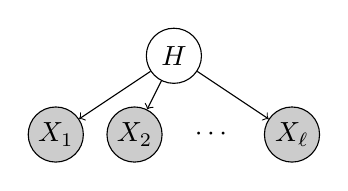
\begin{tikzpicture}
  [
    scale=1.0,
    observed/.style={circle,minimum size=0.7cm,inner sep=0mm,draw=black,fill=black!20},
    hidden/.style={circle,minimum size=0.7cm,inner sep=0mm,draw=black},
  ]
  \node [hidden,name=h] at ($(0,0)$) {$H$};
  \node [observed,name=x1] at ($(-1.5,-1)$) {$X_1$};
  \node [observed,name=x2] at ($(-0.5,-1)$) {$X_2$};
  \node at ($(0.5,-1)$) {$\dotsb$};
  \node [observed,name=xl] at ($(1.5,-1)$) {$X_\ell$};
  \draw [->] (h) to (x1);
  \draw [->] (h) to (x2);
  \draw [->] (h) to (xl);
\end{tikzpicture}}
\hfil\subfigure[Hidden Markov model]{\label{fig:hmm}
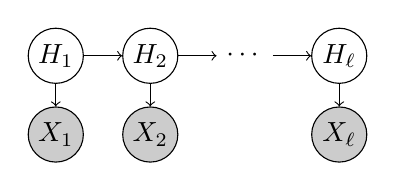
\begin{tikzpicture}
  [
    scale=1.0,
    observed/.style={circle,minimum size=0.7cm,inner sep=0mm,draw=black,fill=black!20},
    hidden/.style={circle,minimum size=0.7cm,inner sep=0mm,draw=black},
  ]
  \node [hidden,name=h1] at ($(-1.2,0)$) {$H_1$};
  \node [hidden,name=h2] at ($(0,0)$) {$H_2$};
  \node [name=hd] at ($(1.2,0)$) {$\dotsb$};
  \node [hidden,name=hl] at ($(2.4,0)$) {$H_\ell$};
  \node [observed,name=x1] at ($(-1.2,-1)$) {$X_1$};
  \node [observed,name=x2] at ($(0,-1)$) {$X_2$};
  \node [observed,name=xl] at ($(2.4,-1)$) {$X_\ell$};
  \draw [->] (h1) to (h2);
  \draw [->] (h2) to (hd);
  \draw [->] (hd) to (hl);
  \draw [->] (h1) to (x1);
  \draw [->] (h2) to (x2);
  \draw [->] (hl) to (xl);
\end{tikzpicture}}
\end{center}
\vspace{-5mm}
\caption{Examples of latent variable models.
}
\label{fig:graphical-model}
\vspace{-1mm}
\end{figure}

Furthermore, in this case, $\widetilde \Ccal_{X|H} = \rbr{\mu_{X|h=1},\ \mu_{X|h=2},\ \ldots,\ \mu_{X|h=k}}$, and the approximate kernel embeddings for $\PP(X_1,X_2)$ and $\PP(X_1,X_2,X_3)$ are 
\begin{align}
  \widetilde \Ccal_{X_1 X_2}
  & = \sum_{h \in [k]} \pi_h \cdot \mu_{X|h} \otimes \mu_{X|h}, \label{eq:joint2} \\
  \widetilde \Ccal_{X_1 X_2 X_3}
  &= \sum_{h \in [k]} \pi_h \cdot \mu_{X|h} \otimes \mu_{X|h} \otimes \mu_{X|h} \label{eq:joint3}
\end{align}
where $\pi_h:=\PP(h)$. 


% Then we can embedding into RKHS the second and third order marginal distribution of the observed variables in the multiview latent variable models in \, \eq{eq:joint2} and \, \eq{eq:joint3}. These kernel embeddings will also factorize according the conditional independence structure of the underlying model. More specifically,
% \begin{align*}
%   \Ccal_{X_1,X_2,X_3}
%   = \EE_{X_1,X_2,X_3}[\phi(X_1)\otimes \phi(X_2) \otimes \phi(X_3)]
% \end{align*}
% Making use of the distribution factorization of the model, we have that
% \begin{align*}
%   \Ccal_{X_1,X_2,X_3} =
%   \sum_{j=1}^k \pi_j \cdot \EE_{X_1| H=j}[\phi(X_1)]\otimes \EE_{X_2|H=j} [\phi(X_2)] \otimes \EE_{X_3|H=j}[\phi(X_3)]
% \end{align*}
% where $\mu_{X_t|j}:=\EE_{X_t| H=j}[\phi(X_t)] = \int_{\Xcal} \phi(X_t)\, d P(X_t|H=j)$ is the
% the conditional embedding of the observed variable $X_t$ given latent variable $H=j$.
% Then we can express the embedding $\Ccal_{X_1,X_2,X_3}$ as a sum of outer product of conditional embeddings, \, \ie,
% \begin{align*}
%   \Ccal_{X_1,X_2,X_3}
%   = \sum_{j=1}^k \pi_j \cdot \mu_{X_1|j} \otimes \mu_{X_2|j} \otimes \mu_{X_3|j}
% \end{align*}
% Similarly, for the joint distribution of the two observed variable in \, \eq{eq:joint2}, we have
% \begin{align*}
%   \Ccal_{X_t,X_{t'}}
%   = \sum_{j=1}^k \pi_j \cdot \mu_{X_t|j} \otimes \mu_{X_{t'}|j},\quad \{t,t'\} \subset \{1,2,3\},\ t\neq t'
% \end{align*}

{\bf Identifiability.} Allman et al. showed that, under mild conditions, a finite mixture of nonparametric product distributions is identifiable. The multiview latent variable model in~\eq{eq:joint3} has the same form as a finite mixture of nonparametric product distribution, and therefore we can adapt Allman's results to the current setting.
\begin{theorem}
  Let $\PP(X_1,X_2,X_3)$ be a multiview latent variable model of the form~\eq{eq:joint3}, such that the conditional distributions $\cbr{\PP(X|h)}_{h \in [k]}$ are linearly independent. Then, the set of parameters $\cbr{\pi_h, \mu_{X|h}}_{h \in [k]}$ are identifiable from $\Ccal_{X_1 X_2 X_3}$, up to label swapping of the hidden variable $H$. 
\end{theorem}

% \section{Whitening with Three Different Views}

% \begin{itemize}
% 	\item $\widetilde{\Ccal}_{12} = \Ccal_{12} \Ucal_2^\top$; $\widetilde{\Ccal}_{13} = \Ccal_{13} \Ucal_3^\top$; $\widetilde{\Ccal}_{23} = \Ucal_{2} \Ccal_{23} \Ucal_3^\top$
% 	\item $\widetilde{\Ccal}_{11} = \widetilde{\Ccal}_{12} (\widetilde{\Ccal}_{32})^{-1} \widetilde{\Ccal}_{31}^\top = \widetilde{\Ucal}_1 \widetilde{\Scal}_1 \widetilde{\Ucal}_1^\top$
% 	\item $\widetilde{\Tcal} = \Ccal_{123} \times_1 (\widetilde{\Ucal}_1 \widetilde{\Scal}_1^{-1/2})^\top  \times_2 (\widetilde{\Ucal}_2 \widetilde{\Scal}_2^{-1/2})^\top \times_3 (\widetilde{\Ucal}_3 \widetilde{\Scal}_3^{-1/2})^\top$
% \end{itemize}

\section{Kernel Algorithm}

We will deal with the discrete latent variable case. 
The parameters $\cbr{\pi_h, \mu_{X|h}}_{h \in [k]}$, of the multiview latent variable model can be recovered from $\Ccal_{X_1 X_2}$ and $\Ccal_{X_1 X_2 X_3}$ using the following simple algorithm.
\begin{enumerate}
  \item Eigen-value decomposition for $\Ccal_{X_1 X_2}$,
    $$\Ccal_{X_1 X_2} = \sum_{i=1}^{\infty} \sigma_i \cdot u_i \otimes u_i$$
    where the eigen-values are ordered in non-decreasing manner. Let the leading $k$ eigenvectors corresponding to the largest $k$ eigen-value be  $\Ucal_k:=(u_1,u_2,\ldots,u_k)$, and the eigen-value matrix of $S_k:=\diag(\sigma_1,\sigma_2,\ldots,\sigma_k)$.
  \item Whiten the 3rd order kernel embedding $\Ccal_{X_1 X_2 X_3}$ using whitening matrix $\Wcal:= \Ucal_k S_k^{-1/2}$.
    $$\Tcal := \Ccal_{X_1 X_2 X_3} \times_1 (\Wcal^\top) \times_2 (\Wcal^\top) \times_3 (\Wcal^\top)$$
    where $\times_i$ denotes mode-$i$ tensor-matrix multiplication.
  \item Find the leading $k$ tensor eigenvectors $V_k$ for $\Tcal$ using tensor power method.
  \item Recover the conditional embedding operator by
    $$ \Ccal_{X|H} = (\mu_{X|h=1},\mu_{X|h=1},\ldots,\mu_{X|h=k}) = (\Wcal)^\dagger V_k $$
\end{enumerate}

{\bf Finite sample estimate.} Given $m$ observation $\Dcal_{X_1 X_2 X_3}=\{(x_1^i,x_2^i,x_3^i)\}_{i \in [m]}$ drawn~\iid~from a multi-view latent variable model $\PP(X_1,X_2,X_3)$, we now design a kernel algorithm to estimate the latent parameters from data. Although the empirical kernel embeddings has infinite dimensions, we can carry out the decomposition using just the kernel matrices.

\begin{enumerate}

\item We will perform a kernel eigenvalue decomposition of the empirical 2nd order embedding 
$$
  \widehat \Ccal_{X_1 X_2}:= \frac{1}{2m} \sum_{i=1}^{m} \rbr{\phi(x_1^i) \otimes \phi(x_2^i) + \phi(x_2^i) \otimes \phi(x_1^i)}.
$$ 
Denote the implicitly formed feature matrix by 
\begin{align*}
  \Phi &:= (\phi(x_1^1),  \phi(x_1^2), \ldots, \phi(x_1^m), \phi(x_2^1),  \phi(x_2^2), \ldots, \phi(x_2^m))  \\
  \Psi &:= (\phi(x_2^1), \phi(x_2^2), \ldots, \phi(x_2^m), \phi(x_1^1),  \phi(x_1^2), \ldots, \phi(x_1^m))  
\end{align*}
respectively, and the corresponding kernel matrix be $K = \Phi^\top \Phi$ and $L = \Psi^\top \Psi$. Using the feature matrix, $\Ccal_{X_1 X_2}$ can be expressed as
$$
	\Ccal_{X_1 X_2} = \frac{1}{2m} \Phi \Psi^\top.
$$
Its leading $k$ eigenvectors $\Ucal_k = (u_1,\ldots,u_k)$ will lie in the span of the column of  $\Phi$,~\ie,~$\Ucal_k = \Phi (\beta_1,\ldots,\beta_k)$ where $\beta \in \RR^m$. Then we can transform the eigen-value decomposition problem for an infinite dimensional matrix to a problem involving finite dimensional kernel matrices,
$$
	\Ccal_{X_1 X_2}\, \Ccal_{X_1 X_2}^\top\, u = \sigma \;u
	\quad \Rightarrow \quad
	\frac{1}{4m^2}\Phi \Psi^\top \Psi \Phi^\top \Phi \beta = \sigma\,\Phi \beta
	\quad \Rightarrow \quad
	\frac{1}{4m^2} K L K \beta = \sigma \,K \beta.
$$
Let the Cholesky decomposition of $K$ be $R^\top R$. Then by redefining $\widetilde{\beta}=R\beta$, and solving an eigenvalue problem
\begin{align}
 \frac{1}{4m^2} R L R^\top \widetilde{\beta} = \sigma \, \widetilde{\beta},~~\text{and obtain}~\beta = R^{\dagger} \widetilde{\beta}.
\end{align}
The resulting eigenvectors satisfy $u_i^\top u_{i'} = \beta_i^\top \Phi^\top \Phi \beta_{i'} =  \beta_{i}^\top K  \beta_{i'} =  \widetilde{\beta}_{i}^\top \widetilde{\beta}_{i'}=\delta_{ii'}$.
This algorithm is summarized in Algorithm~\ref{alg:svd}. 

\begin{algorithm}[t!]
\caption{KernelSVD($K$, $L$, $k$)}
% 	\textbf{In}: Two kernel matrices $K$ and $L$, and desired rank $r$ \\
	\textbf{Out}: $S_k$ and $(\beta_1,\ldots,\beta_k)$\\[-0.4cm]
  \begin{algorithmic}[1]
    \STATE Perform Cholesky decomposition:\ $K=R^\top R$
    \STATE Solve eigen-decomposition problem:\ $\frac{1}{4m^2} R L R^\top \widetilde{\beta} = \sigma\,\widetilde{\beta}$
    \STATE Let the $k$ leading eigen-values be:\ $S_k = \diag(\sigma_1,\ldots,\sigma_k)$
    \STATE Let the corresponding $k$ leading eigenvectors be:\ $(\widetilde{\beta}_1,\ldots,\widetilde{\beta}_k)$
    \STATE Compute:\ $(\beta_1,\ldots,\beta_k) = R^\dagger (\widetilde{\beta}_1,\ldots,\widetilde{\beta}_k)$
% 		, and reorgnaize $(\thetab^1,\ldots,\thetab^n)^\top = (\beta_1,\ldots,\beta_k)$
  \end{algorithmic}
  \label{alg:svd}
\end{algorithm}

\item We whiten the empirical 3rd order embedding 
$$
  \widehat \Ccal_{X_1 X_2 X_3}:=\frac{1}{3m}\sum_{i=1}^{m} \rbr{\phi(x_1^i) \otimes \phi(x_2^i) \otimes \phi(x_3^i) + \phi(x_3^i) \otimes \phi(x_1^i) \otimes \phi(x_2^i) + \phi(x_2^i) \otimes \phi(x_3^i) \otimes \phi(x_1^i)}
$$ 
to obtain
\begin{align}
  \widehat \Tcal := \frac{1}{3m}\sum_{i=1}^m \rbr{\xi(x_1^i) \otimes \xi(x_2^i) \otimes \xi(x_3^i) + \xi(x_3^i) \otimes \xi(x_1^i) \otimes \xi(x_2^i) + \xi(x_2^i) \otimes \xi(x_3^i) \otimes \xi(x_1^i)},
\end{align}
where
$$
	\xi(x_1^i) := S_k^{-1/2} (\beta_1,\ldots,\beta_k)^\top \Phi^\top \phi(x_1^i)\quad \in \quad \RR^k.
$$

\item We run tensor power method in Algorithm~\ref{alg:robustpower} on the finite dimension tensor $\widehat \Tcal$ to obtain its leading $k$ eigenvectors $V_k:=(v_1,\ldots,v_k)$. 

\item The estimate for the conditional embedding is given by
\begin{align}
  \widehat \Ccal_{X|H} = (\widehat \mu_{X|h=1},\ldots, \widehat \mu_{X|h=k}) = \Phi (\beta_1,\ldots,\beta_k) S_k^{1/2} V_k
\end{align}

\end{enumerate}

\section{Interpretation with Parametric Family}

For interpretable results, we can project the nonparametric representation to parametric family of distributions (\eg, \, exponential families) as post-processing.

\section{Sample Complexity Analysis}

\subsection{Robust Tensor Power Method}
We recap the robust tensor power method for finding the tensor eigen-pairs, analyzed in detail in~\cite{AnandkumarEtal:community12}.

\begin{algorithm}
\caption{$\{\lambda, \Phi\}\leftarrow $TensorEigen$(T,\, \{v_i\}_{i\in [L]}, N)$}\label{alg:robustpower}
\begin{algorithmic}
\renewcommand{\algorithmicrequire}{\textbf{Input: }}
\renewcommand{\algorithmicensure}{\textbf{Output: }}
\REQUIRE Tensor $T\in \R^{k \times k \times k}$, set of $L$ initialization vectors $\{v_i\}_{i\in L}$, number of
iterations  $N$.
%\ENSURE Eigenpairs:  $\lambda$ is the vector of eigenvalues and $\Phi$ is the matrix of eigenvectors of  $T$.
\ENSURE the estimated eigenvalue/eigenvector pairs $\{\lambda, \Phi\}$, where $\lambda$ is the vector of eigenvalues and $\Phi$ is the matrix of eigenvectors.

\FOR{$i =1$ to $k$}
\FOR{$\tau = 1$ to $L$}
\STATE $\th{0}\leftarrow v_\tau$.
\FOR{$t = 1$ to $N$}
\STATE $\tilde{T}\leftarrow T$.
\FOR{$j=1$ to $i-1$ (when $i>1$)}
\IF{$|\lambda_j \inner{\th{t}^{(\tau)}, \phi_j}|>\xi$}
\STATE $\tilde{T}\leftarrow \tilde{T}- \lambda_j \phi_j^{\otimes 3}$.
\ENDIF
\ENDFOR

\STATE Compute power iteration update
$
\th{t}^{(\tau)}  :=
\frac{\tilde{T}(I, \th{t-1}^{(\tau)}, \th{t-1}^{(\tau)})}
{\|\tilde{T}(I, \th{t-1}^{(\tau)}, \th{t-1}^{(\tau)})\|}
$\ENDFOR
\ENDFOR

\STATE Let $\tau^* := \arg\max_{\tau \in L} \{ \tilde{T}(\th{N}^{(\tau)},
\th{N}^{(\tau)}, \th{N}^{(\tau)}) \}$.

\STATE Do $N$ power iteration updates starting from
$\th{N}^{(\tau^*)}$ to obtain eigenvector estimate $\phi_i$, and set $\lambda_i :=
\tilde{T}(\phi_i, \phi_i, \phi_i)$.

\ENDFOR
\RETURN the estimated eigenvalue/eigenvectors
$(\lambda, \Phi)$.

\end{algorithmic}
\end{algorithm}


We now recap the result of~\cite[Thm. 13]{AnandkumarEtal:community12} that establishes bounds on the eigen-estimates under good initialization vectors for the above procedure. 
Let $\Tcal=\sum_{i\in [k]}\lambda_i v_i$, where $v_i$ are orthonormal vectors and $\lambda_1\geq \lambda_2\geq\ldots \lambda_k$. Let $\h{\Tcal}=\Tcal+E$ be the perturbed tensor with $\|E\|\leq \epsilon_{T}$. Recall that $N$ denotes the number of iterations of the tensor power method.
We call an initialization vector $u$ to be $(\gamma, R_0)$-good  if there exists $v_i$ such that $\inner{u, v_i}> R_0$
  and $|\inner{u, v_i}| -\max_{j<i} |\inner{u,v_j}| > \gamma  |\inner{u,v_i}|$.   Choose $\gamma=1/100$.


\begin{theorem}
\label{thm:robustpower}
There exists universal constants $C_1, C_2 > 0$  such that the
following holds.
\beq\label{eqn:robustpowerconditions}
\epsilon_{T} \leq C_1 \cdot \lambda_{\min} R_0^2,
\qquad
N \geq C_2 \cdot \left( \log(k) + \log\log\left(
\frac{\lambdamax}{\epsilon_{tensor}} \right) \right)
,
\eeq Assume there is at least one good initialization vector corresponding to each $v_i$, $i\in [k]$. The parameter $\xi$ for choosing deflation vectors in each iteration of the tensor power method in Procedure~\ref{alg:robustpower}  is chosen as $\xi\geq 25 \eps$. We obtain  eigenvalue-eigenvector pairs  $(\hat\lambda_1,\hat{v}_1), (\hat\lambda_2,\hat{v}_2), \dotsc,
(\hat\lambda_k,\hat{v}_k)$ such that  there exists a permutation $\pi$ on
$[k]$ with
\[
\|v_{\pi(j)}-\hat{v}_j\| \leq 8 \epsilon/\lambda_{\pi(j)}
, \qquad
|\lambda_{\pi(j)}-\hat\lambda_j| \leq 5\epsilon , \quad \forall j \in [k]
,
\]
and
\[
\left\|
\Tcal - \sum_{j=1}^k \hat\lambda_j \hat{v}_j^{\otimes 3}
\right\| \leq 55\eps .
\]
\end{theorem}

In the sequel, we establish concentration bounds that allows us to translate the above condition on tensor perturbation~\eqref{eqn:robustpowerconditions}  to sample complexity bounds.

\subsection{Concentration Bounds}

\subsubsection{Analysis of Whitening} 

Recall that we use the covariance operator $\Ccal_{X_1 X_2}$ for whitening the 3rd order embedding $\Ccal_{X_1, X_2, X_3}$. We first analyze the perturbation in whitening when sample estimates are employed. 

Let $\h{\Ccal}_{X_1 X_2}$ denote the sample covariance operator between variables $X_1$ and $X_2$, and let \[B:=0.5(\h{\Ccal}_{X_1 X_2}+ \h{\Ccal}_{X_1 X_2}^\top)=\h{\Ucal}\h{S}\h{\Ucal}^\top\] denote the SVD.
Let $\Ucal_k$ and $S_k$ denote the restriction to top-$k$ eigen-pairs, and let $B_{k} := \Ucal_k S_k \Ucal_k^\top$. Recall that the whitening matrix is given by $\h{\Wcal}:=\h{\Ucal}_k \h{S}_k^{-1/2}$. Now $\h{\Wcal}$ whitens $B_k$, i.e. $\h{\Wcal}^\top B_{k} \h{\Wcal}=I$.

Now consider the SVD of
\[ \h{\Wcal}^\top \Ccal_{X_1 X_2} \h{\Wcal}= A D A^\top,\] and define \[\Wcal:= \h{\Wcal} AD^{-1/2}A^\top, \] and $\Wcal$ whitens $\Ccal_{X_1 X_2}$ since $\Wcal^\top  \Ccal_{X_1 X_2} W=I$.
Recall that by exchangeability assumption, 
\[ \Ccal_{X_1,X_{2}}
  = \sum_{j=1}^k \pi_j \cdot \mu_{X|j} \otimes \mu_{X|j} \tcr{+  E_{X_1 X_2}}= M \Diag(\pi) M^\top  \tcr{+E_{X_1 X_2}}, \] where the $j^{\tha}$ column of $M$, $M_j = \mu_{X|j}$.

We now establish the following perturbation bound on the whitening procedure. Recall from \eqref{eqn:deltapairs}, $ \epsilon_{pairs}:=\nbr{\Ccal_{X_1,X_{2}} - \widehat \Ccal_{X_1,X_{2}}}_{}$. Let $\sigma_1(\cdot) \geq \sigma_2(\cdot)\ldots$ denote the singular values of an operator.

\begin{lemma}[Whitening perturbation]\label{lemma:whiten} Assuming that $\epsilon_{pairs} < 0.5 \sigma_k(\Ccal_{X_1 X_2})$,
\beq \epsilon_{W}:= \|\Diag(\pi)^{1/2}M^\top(\h{\Wcal}-\Wcal)\|\leq \frac{2(2\epsilon_{pairs} \tcr{+\sigma_{k+1}(\Ccal_{X_1 X_2})})}{ \sigma_{k}(\Ccal_{X_1 X_2})}\tcr{\cdot (1+ \sigma_{k+1}(\Ccal_{X_1 X_2}))}\eeq
\end{lemma}

\paragraph{Remark: }Note that $\sigma_{k}(\Ccal_{X_1 X_2}) = \sigma_{k}^2(M)$.

\bprf The proof is along the lines of~\cite[Lemma 16]{AnandkumarEtal:community12}, but adapted to whitening using the covariance operator here.
 \begin{align*}\|\Diag(\pi)^{1/2} M^\top(\h{\Wcal}-\Wcal)\|&= 
\|\Diag(\pi)^{1/2} M^\top W(A D^{1/2} A^\top -I)\|\\ &\leq\|\Diag(\pi)^{1/2} M^\top \Wcal\| \|D^{1/2}-I\|. \end{align*} Since $\Wcal$ whitens $\Ccal_{X_1 X_2}=M \Diag(\pi) M^\top\tcr{+E}$, we have that $\|\Diag(\pi)^{1/2} M^\top \Wcal\|=1$ \tcr{or $\|\Diag(\pi)^{1/2} M^\top \Wcal\|\leq \|I-E\|^{1/2}\leq 1+ \sigma_{k+1}(\Ccal_{X_1 X_2})$}. Now we control $\|D^{1/2}-I\|$.  Let $\tl{E}:= \Ccal_{X_1,X_{2}} -B_k$, where recall that $B=0.5( \widehat \Ccal_{X_1,X_{2}}+ \h{\Ccal}_{X_1 X_2}^\top)$ and $B_k$ is its restriction to top-$k$ singular values. Thus, we have $\|\tl{E}\|_{HS} \leq \epsilon_{pairs} + \sigma_{k+1}(B)\leq 2\epsilon_{pairs}\tcr{+\sigma_{k+1}(\Ccal_{X_1 X_2})} $.
 We now have
\begin{align*}
\|D^{1/2}-I\|&\leq \|(D^{1/2}-I)(D^{1/2}+I)\|\leq \|D-I\|
\\ &=\|AD A^\top - I\| = \|\h{\Wcal}^\top \Ccal_{X_1 X_2}  \h{\Wcal} -I\|\\ &=\| \h{\Wcal}^\top  \tl{E} \h{\Wcal}\| \leq \|\h{\Wcal}\|^2 ( 2 \epsilon_{pairs}\tcr{+\sigma_{k+1}(\Ccal_{X_1 X_2})}).
\end{align*}Now
\[ \|\h{\Wcal}^2\| \leq\frac{1}{ \sigma_k(\h{\Ccal}_{X_1 X_2})}\leq \frac{2}{\sigma_k(\Ccal_{X_1 X_2})},\] when  $\epsilon_{pairs}<0.5 \sigma_k(\Ccal_{X_1 X_2})$.
\eprf

\subsubsection{Tensor Concentration Bounds}

Recall that the whitened tensor from samples is given by
$$\h{\Tcal} := \h{\Ccal}_{X_1 X_2 X_3} \times_1 (\h{\Wcal}^\top) \times_2 (\h{\Wcal}^\top) \times_3 (\h{\Wcal}^\top).$$ We want to establish its perturbation from the whitened tensor using exact statistics
$$\Tcal := \Ccal_{X_1 X_2 X_3} \times_1 (\Wcal^\top ) \times_2 (\Wcal^\top ) \times_3 (\Wcal^\top ).$$ Further, we have 
$$\Ccal_{X_1 X_2 X_3}= \sum_{h\in [k]} \pi_h \cdot \mu_{X|h} \otimes \mu_{X|h} \otimes \mu_{X|h} \tcr{+ E_{X_1, X_2, X_3}}$$

Let $\epsilon_{triples}:= \|\h{\Ccal}_{X_1 X_2 X_3}-\Ccal_{X_1 X_2 X_3}\|_{}$. Let $\pi_{\min}:=\min_{h\in [k]}\pi_h$.

\begin{lemma}[Tensor perturbation bound]
Assuming that $\epsilon_{pairs} < 0.5 \sigma_k(\Ccal_{X_1 X_2})$, we have
\beq\label{eqn:epsilonT} \epsilon_T:= \|\h{\Tcal} - \Tcal\|
\leq \frac{2\sqrt{2}\epsilon_{triples}}{\sigma_k(\Ccal_{X_1 X_2})^{1.5} }+\frac{\epsilon_W^3}{\sqrt{\pi_{\min}}}
\tcr{+ \|E_{X_1 X_2 X_3}\| \frac{\epsilon_W^3}{\pi_{\min}^{1.5} \sigma_k(M)^3} }.\eeq
\end{lemma} 


\bprf  Define
  intermediate tensor
\begin{align*} \tl{\Tcal}&:= \Ccal_{X_1 X_2 X_3} \times_1 (\h{\Wcal}^\top) \times_2 (\h{\Wcal}^\top) \times_3 (\h{\Wcal}^\top).\end{align*}
We will bound $\|\h{\Tcal}-\tl{\Tcal}\|$  and $\| \h{\Tcal}-\Tcal\|$  separately. 
\begin{align*}
\|\h{\Tcal}-\tl{\Tcal}\| &\leq \|\h{\Ccal}_{X_1, X_2, X_2} - \Ccal_{X_1, X_2, X_3}\| \|\h{\Wcal}\|^3\leq \frac{2\sqrt{2}\epsilon_{triples}}{\sigma_k(\Ccal_{X_1 X_2})^{1.5} },
\end{align*}using the bound on $\|\h{\Wcal}\|$ in Lemma~\ref{lemma:whiten}. For the other term,
first note that
\[ \Ccal_{X_1, X_2, X_3} = \sum_{h\in [k]} \pi_h \cdot M_h \otimes M_h \otimes M_h \tcr{+ E_{X_1, X_2, X_3}}, \]
 \tcr{ where $\|E_{X_1, X_2, X_3}\|$ is the residual and we need to bound this in non-parametric case.}
\begin{align*} \|\h{\Tcal}-\Tcal\|&= \| \Ccal_{X_1 X_2 X_3}\times_1 (\h{\Wcal} -\Wcal)^\top \times_2 (\h{\Wcal} -\Wcal)^\top \times_3 (\h{\Wcal}-\Wcal)^\top\| \\
&\leq \frac{ \| \Diag(\pi)^{1/2}M^\top(\h{\Wcal}-\Wcal)\|^3}{\sqrt{\pi_{\min}}}
\tcr{+ \|E_{X_1 X_2 X_3}\| \|\h{\Wcal}-\Wcal\|^3}\\
&= \frac{\epsilon_W^3}{\sqrt{\pi_{\min}}}
\tcr{+ \|E_{X_1 X_2 X_3}\| \frac{\epsilon_W^3}{\pi_{\min}^{1.5} \sigma_k(M)^3} }
\end{align*}
\eprf\\


We obtain a condition on the above perturbation $\epsilon_T$ in \eqref{eqn:epsilonT} by applying Theorem~\ref{thm:robustpower} as
$ \epsilon_T\leq C_1\lambda_{\min} R_0^2$. Here, we have $\lambda_{i} = 1/\sqrt{\pi_{i}}\geq 1$. For random initialization, we have that $R_0 \sim 1/\sqrt{k}$, with probability $1-\delta$ using $\poly(k) \poly(1/\delta)$ trials~\cite[Thm. 5.1]{AnandkumarEtal:tensor12}. Thus, we require that $ \epsilon_T  \leq \frac{C_1}{k}$. Summarizing, we require for the following conditions to hold 
\beq\epsilon_{pairs}\leq 0.5 \sigma_k(\Ccal_{X_1 X_2}), \quad \epsilon_T  \leq \frac{C_1}{k}.\eeq

\aacomment{need to substitute for $\epsilon_{pairs}$ and $\epsilon_{triples}$ and if we bound the residuals, we are done.}

\subsubsection{Concentration bounds for Empirical Operators}

Concentration results for the singular value decomposition of empirical operators.

\begin{lemma} Let $\kappa:=\sup_{x \in \Omega} k(x,x)$, and $\| \cdot\|_{}$ be the Hilbert-Schmidt norm, we have for \beq \epsilon_{pairs}:=\nbr{\Ccal_{X_1 X_2} - \widehat \Ccal_{X_1 X_2}}_{},\label{eqn:deltapairs} \eeq
\begin{eqnarray}
	\Pr \cbr{\epsilon_{pairs}  \leqslant \frac{2\sqrt{2}\kappa \sqrt{\delta}}{\sqrt{m}} } \geqslant 1-2\exp(-\delta). \label{eq:operator_concentration}
\end{eqnarray}
\end{lemma}

\begin{proof}
We will use similar arguments as in~\cite{RosBelVit2010} which deals with symmetric operator. Let $\xi_{i}$ be defined as
\begin{eqnarray}
\xi_{i}\, =\, \phi(x_t^i) \otimes \phi(x_{t'}^i) - \Ccal_{X_t,X_{t'}}.
\end{eqnarray}
It is easy to see that $\mathbb{E}[\xi_{i}] = 0$. Further, we have
\begin{eqnarray}
	\sup_{x_1,x_2} \nbr{\phi(x_1) \otimes \phi(x_2)}^{2}_{} \leqslant \kappa^{2},
\end{eqnarray}
which implies that $\nbr{\Ccal_{X_1 X_2}}_{} \leqslant \kappa$, and $\nbr{\xi_i}_{} \leqslant 2 \kappa$. The result then follows from the Hoeffding's inequality in Hilbert space.
\end{proof}

Similarly, we have the concentration bound for 3rd order embedding

\begin{lemma} Let $\kappa:=\sup_{x \in \Omega} k(x,x)$, and $\| \cdot\|_{}$ be the Hilbert-Schmidt norm, we have for \beq \epsilon_{pairs}:=\nbr{\Ccal_{X_1 X_2 X_3} - \widehat \Ccal_{X_1 X_2 X_3}}_{},\label{eqn:deltapairs} \eeq
\begin{eqnarray}
	\Pr \cbr{\epsilon_{triples}  \leqslant \frac{3\sqrt{2}\kappa \sqrt{\delta}}{\sqrt{m}} } \geqslant 1-2\exp(-\delta). \label{eq:operator_concentration2}
\end{eqnarray}
\end{lemma}

\bibliographystyle{unsrt}
\bibliography{nonparametric_mixture,bibfile}
% {../../../newbibfile/bibfile} % L
% \bibliography{../../../../newbibfile/bibfile} % L

\end{document}

%%%%%%%%%%%%%%%%%%%%%%%%%%%%%%%%%%
%%%%%%%%%%%%%%%%%%%%%%%%%%%%%%%%%%
%%%%%%%%%%%%%%%%%%%%%%%%%%%%%%%%%%


